\section{Introduction}
\label{sec:intro}



Mental health, a critical facet of overall well-being, remains a global challenge affecting individuals from diverse backgrounds \cite{Dreisbach2019systematic}. 
% According to the National Institute of Mental Health report of 2021, there were an estimated 57.8 million adults in the United States with Any Mental Illness (AMI) and an estimated 14.1 million adults with Serious Mental Illness (SMI)\footnote{\url{https://www.nimh.nih.gov/health/statistics/mental-illness}}.
Traditional methods for studying mental health have often relied on clinical assessments, surveys, and interviews \cite{beck1996beck}, providing valuable but limited snapshots of an individual's mental state. Mental disorders often manifest as long-term conditions, unfolding gradually over extended periods \cite{collingridge2010long}. This intrinsic characteristic of mental health issues presents a challenge to current clinical diagnosis and assessment methods, which predominantly concentrate on symptom duration within a narrow two-week window \cite{american2013diagnostic}. Such an approach may not fully capture the nuanced and evolving nature of mental illnesses, potentially overlooking the progressive development of symptoms and the broader impact on an individual's life. 
\begin{figure}[th]
	\centering
	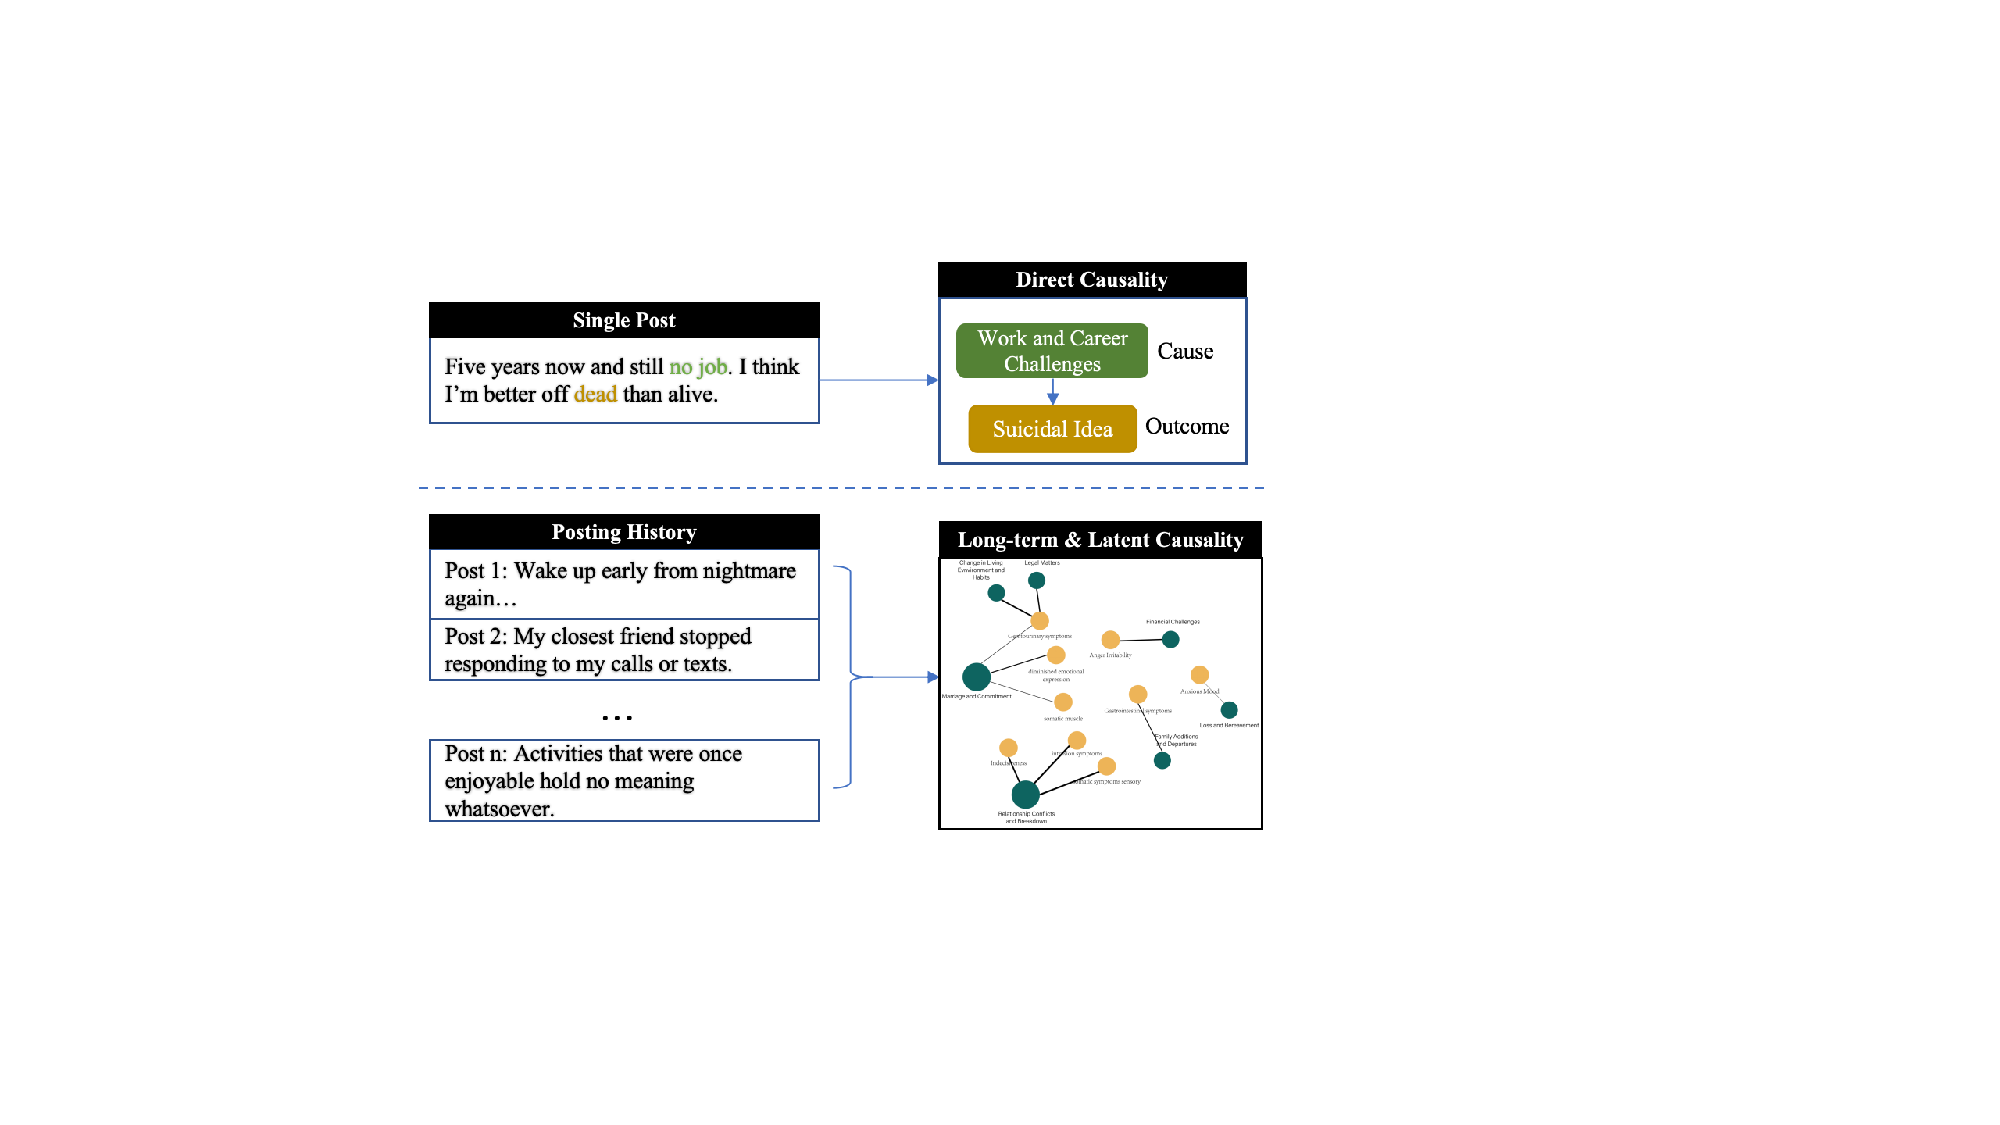
\includegraphics[width=\linewidth]{figures/overview.pdf}
	\caption{Direct causal relationships from a single post (above) versus long-term and latent causality from a multi-post history (below).}
	\label{fig:overview}
\end{figure}

This discrepancy highlights the need for a more longitudinal perspective in mental health assessment, one that considers the full spectrum of symptom development and progression over time, thereby providing a more accurate and holistic view of an individual’s mental health state.
To this end, social media platforms serve as a valuable resource for tracking mental health, 
with users frequently documenting their thoughts and emotions over extended periods. 
In contrast to traditional clinical methods that focus on short-term symptoms, 
social media posts offer a continuous, candid narrative of an individual's mental state. 
This user-generated content provides insights into the evolving nature of mental health, 
capturing subtle changes and patterns over time that might be overlooked in brief 
clinical assessments. 
%Thus, social media presents a more dynamic and holistic view of individual mental well-being.
Discussions about symptoms and life stressors on social media are closely tied to mental 
well-being~\cite{charles2013wear,harandi2017correlation}. 
Monitoring the evolution of users' posts over time enables a more comprehensive 
analysis of the origins and progression of their conditions, 
facilitating early interventions when signs of mental health issues emerge.

Previous studies~\cite{shen2017detecting,zhang2022psychiatric} have consistently focused on detecting mental disorders through the textual content of social media posts, neglecting the analysis of chronological attributes. While achieving high detection accuracy~\cite{chancellor2020methods, chen-etal-2023-detection}, we argue that a singular outcome is insufficient for a profound comprehension of mental disorder development and the relationships among various factors (e.g., psychiatric symptoms). Recently, some pioneering studies \cite{garg2022cams, Saxena2023Explainable} began to explore the causes of mental health issues in social media posts.  
Nevertheless, their focus remains solely on extracting \textit{direct} causal relationships from the semantic information within one post~\cite{luo2016commonsense}, as illustrated in Figure \ref{fig:overview}. This approach can only capture limited causality, as a substantial number of \textit{long-term}, \textit{latent} causal relationships may not necessarily manifest within a single post.

Therefore, our work seeks to address these limitations by revealing latent causes behind psychiatric symptoms through a computational method encompassing users' entire posting history. 
Building upon existing literature that indicates reciprocal influences among symptoms \cite{Gulistan2021Signal, Anish2023Mental} and the potential for stressful life events to cause symptoms \cite{Radell2021Abuse, Ruengorn2021Association}, we endeavor to explore both ``\textit{symptom-to-symptom}'' and ``\textit{life-event-to-symptom}'' causal relationships in this research. 

We conduct our analysis on a large-scale dataset of Reddit posts with users diagnosed with various mental disorders \cite{chen-etal-2023-detection}. 
% The text-based nature of our dataset introduces complexity compared to non-text datasets, necessitating sophisticated modeling to capture semantically meaningful factors~\cite{Feder2022Causal}.\MY{Every paragraph should have a clear focus, every sentence serves this purpose. This sentence is distracted, no need to keep, consider deleting it. We are not comparing our work to any other source formats.}
Our initial step involves training models to identify psychiatric symptoms and life events\footnote{We identify 38 symptoms, such as depressed mood, poor memory, etc., and 11 life events, including financial challenges \cite{Noone2017stress,Zhang2022SymptomIF}. The complete list is provided in Appendix \ref{sec:appendixA}.} from our text dataset. 
Then, we employ the classical causal discovery method, propensity score matching (PSM)~\cite{Rosenbaum1983TheCR}, to unveil the causal relationships between the past symptoms or life events and the future symptoms. 
To illustrate the efficacy of causality unveiled from social media posts, we anchor our findings in authoritative psychiatry literature, and find that our results aligns with many clinically controlled experiments. Furthermore, we integrate these identified causal relationships as additional features into two chronological disease detection tasks, namely diagnosis point detection and early risk detection of depression. The enhanced detection performance also underscores the importance of causality.
% \MY{Restate: Causal relations extracted using social media text are in fact supporting by existing clinical controlled experiments, indicating the efficacy of such causality. Further, we identified two chronological disease detection tasks, namely diagnosis point detection and early detection of depression, with increased detection accuracy demonstrating the importance of causality.}
The main contributions of this work are:
\begin{itemize}
    % \item We highlight the limitations of narrowly focusing on disease detection tasks\MY{This one doesn't make sense -> it's not the task focus is narrow, but we are advocating for a temporal perspective towards mental disorder detection. We extract these causal features and find them helpful in disease detection, in particular  early detection and diagnosis time prediction}. We urge for greater attention to the dynamically evolving nature of mental health issues, to achieve a more comprehensive understanding of their causes and progression.
    % \item We utilized propensity score matching on social media posts to uncover latent and long-term causal relationships of diverse factors related to mental disorders (i.e., psychiatric symptoms and life events), addressing the limitations of direct causal relationships in previous works \cite{garg2022cams}\MY{what's direct causal? We don't want to introduce new arguments in contribution part.}.
    % \item We apply these extracted causal relationships to disease detection tasks to fill gaps in the incomplete symptom sequences, thereby boosting the overall performance by xxx. \MY{Your contributions are straightforward: 1. the nuance in causal relations in mental disorder detection via social media posts; 2. Using PSM to extract two different causality and some are supported by existing clinical evidence. 3. These features are found beneficial to detection and prediction tasks, hence working as effective features}
    \item We propose to mine implicit, subtle, and long-term causal relationships between factors related to mental disorders from the enormous and evolving social media stream, which can overcome the limitation of single text extraction methods \cite{garg2022cams}.

    \item We discover various reliable \textit{``symptom-to-symptom''} and \textit{``life event-to-symptom''} causal effects with Propensity Score Matching, which can be supported by existing clinical evidence.

    \item We achieve a significant performance boost in the Early Risk Detection and Diagnosis Point Detection task by applying these extracted causal relationships, which further verify their reliability and efficacy.
\end{itemize}



% \begin{itemize}
%     \item We introduce causality into mental health analysis and study the interaction between symptoms.We obtain the Average Causal Effect(ATE) between pairs of 38 symptoms.
%     \item We study the effect of diverse factors(e.g.,causality,life events) on symptoms and it can help us attain a more profound comprehension of mental illness. 
%     \item We apply these extracted causality features to tasks such as diagnosis point detection and symptom sequence prediction.
% \end{itemize}


% Existing literature suggests reciprocal influences among symptoms (e.g., insomnia potentially leading to memory decline \cite{}). Moreover, life events (e.g., family additions and departures) have also been linked to symptoms \cite{}.  Therefore, our focus is to 


% Semantic attributes exist in social media posts.By analyzing these semantic contents,we can diagnose mental illness. However, there are also temporal attributes between posts.Previous studies have mainly focused on the semantic content of these social media data, overlooking the importance of their temporal attributes.

% External events, personal milestones, or even routine occurrences can impact individuals' mental well-being. Time attributes are essential for uncovering the relationships between these events and emotional shifts. By ignoring time attributes, researchers might fail to identify triggers or falsely associate emotional changes with unrelated factors, leading to misguided insights.

% Furthermore, one of the most detrimental effects of disregarding temporal attributes is the potential for delayed interventions.Without the ability to track these changes in real time, there is a risk of missing critical moments when individuals need immediate support and delayed interventions can exacerbate distress and hinder recovery.Neglecting time attributes between social media posts in mental health analysis hampers the accuracy, depth, and effectiveness of the insights gained.To fully comprehend the progression of mental problems, it is imperative to incorporate this temporal attributes into research and interventions.

% To address these limitations,we introduce causality into mental health analysis.Considering that there may be mutual influence among some symptoms(such as insomnia may cause decline of memory),we try to analyze the relationship between symptoms from the time dimension on existing datasets.We set the symptoms in the current post as the cause and set the length of the sliding window as W.Then we observe the symptoms in the posts in the next W days.By analyzing these posts,we can investigate the causal connections between diverse factors.

% We extract life events in social media posts and study causality between symptoms and life eventscWe utilize propensity score matching(PSM) to uncover the causality between symptoms and life events and the causality among different symptoms.In addition, we apply these extracted causality features to diagnosis point detection and symptom sequence prediction.Given the sequence of symptoms that appeared in the previous period of time,the task of symptom sequence prediction is to predict the symptoms that may occur in the following period.According to experimental results,the effect of diagnosis point detection and symptom sequence prediction has been improved after adding causality.This implies that incorporating causality information can enhance the effect of mental disorder diagnosis and treatment planning.
